\documentclass[12pt,a4paper,twoside,openright]{report}
% CREATED BY DAVID FRISK, 2016

% BASIC SETTINGS
\usepackage{moreverb}								% List settings
\usepackage{textcomp}								% Fonts, symbols etc.
\usepackage{lmodern}								% Latin modern font
\usepackage{helvet}									% Enables font switching
\usepackage[T1]{fontenc}							% Output settings
\usepackage[english]{babel}							% Language settings
\usepackage[utf8]{inputenc}							% Input settings
\usepackage{amsmath}								% Mathematical expressions (American mathematical society)
\usepackage{amssymb}								% Mathematical symbols (American mathematical society)
\usepackage{graphicx}								% Figures
\usepackage{subfig}									% Enables subfigures
\numberwithin{equation}{chapter}					% Numbering order for equations
\numberwithin{figure}{chapter}						% Numbering order for figures
\numberwithin{table}{chapter}						% Numbering order for tables
\usepackage{minted}						    		% Enables source code listings
\usepackage{chemfig}								% Chemical structures
\usepackage[top=3cm, bottom=3cm,
			inner=3cm, outer=3cm]{geometry}			% Page margin lengths			
\usepackage{eso-pic}								% Create cover page background
\newcommand{\backgroundpic}[3]{
	\put(#1,#2){
	\parbox[b][\paperheight]{\paperwidth}{
	\centering
	\includegraphics[width=\paperwidth,height=\paperheight,keepaspectratio]{#3}}}}
\usepackage{float} 									% Enables object position enforcement using [H]
\usepackage{parskip}								% Enables vertical spaces correctly 
\usepackage{datetime} %date formatting tools


% OPTIONAL SETTINGS (DELETE OR COMMENT TO SUPRESS)

% Disable automatic indentation (equal to using \noindent)
\setlength{\parindent}{0cm}                         


% Caption settings (aligned left with bold name)
\usepackage[labelfont=bf, textfont=normal,
			justification=justified,
			singlelinecheck=false]{caption} 		

		  	
% Activate clickable links in table of contents  	
\usepackage{hyperref}								
\hypersetup{colorlinks, citecolor=black,
   		 	filecolor=black, linkcolor=black,
    		urlcolor=black}


% Define the number of section levels to be included in the t.o.c. and numbered	(3 is default)	
\setcounter{tocdepth}{5}							
\setcounter{secnumdepth}{5}	


% Chapter title settings
\usepackage{titlesec}		
\titleformat{\chapter}[display]
  {\Huge\bfseries\filcenter}
  {{\fontsize{50pt}{1em}\vspace{-4.2ex}\selectfont \textnormal{\thechapter}}}{1ex}{}[]


% Header and footer settings (Select TWOSIDE or ONESIDE layout below)
\usepackage{fancyhdr}								
\pagestyle{fancy}  
\renewcommand{\chaptermark}[1]{\markboth{\thechapter.\space#1}{}} 


% Select one-sided (1) or two-sided (2) page numbering
\def\layout{2}	% Choose 1 for one-sided or 2 for two-sided layout
% Conditional expression based on the layout choice
\ifnum\layout=2	% Two-sided
    \fancyhf{}			 						
	\fancyhead[LE,RO]{\nouppercase{ \leftmark}}
	\fancyfoot[LE,RO]{\thepage}
	\fancypagestyle{plain}{			% Redefine the plain page style
	\fancyhf{}
	\renewcommand{\headrulewidth}{0pt} 		
	\fancyfoot[LE,RO]{\thepage}}	
\else			% One-sided  	
  	\fancyhf{}					
	\fancyhead[C]{\nouppercase{ \leftmark}}
	\fancyfoot[C]{\thepage}
\fi


% Enable To-do notes
\usepackage[textsize=tiny]{todonotes}   % Include the option "disable" to hide all notes
\setlength{\marginparwidth}{2.5cm} 


% Supress warning from Texmaker about headheight
\setlength{\headheight}{15pt}		





\newcommand{\oneLineTitle}{A Chalmers University of Technology Master's thesis template for \LaTeX}
\newcommand{\multiLineTitle}[1]{A Chalmers University of Technology \\[#1]  Master's thesis template for \LaTeX}
% The term [#1] indicates that there will be 1 rowbreak to split the title into two pieces, first part before \\[#1] and second part after. If you have a very long title and need to split it up into 3 rows, just use \\[#1] multiple times.

\newcommand{\oneLineSubtitle}{A Subtitle that can be Very Much Longer if Necessary}


\begin{document} 

% COVER PAGE, TITLE PAGE AND IMPRINT PAGE
\pagenumbering{roman}			% Roman numbering (starting with i (one)) until first main chapter
% CREATED BY DAVID FRISK, 2016
% MODIFIED BY JAKOB JARMAR, 2016
% A few changes by Birgit Grohe, 2017 and \the\year
% Adjustments with the help of Gustav Örtenberg 2019

% COVER PAGE
\begin{titlepage}
\newgeometry{top=3cm, bottom=3cm,
			left=2.25 cm, right=2.25cm}	% Temporarily change margins		
			
% Cover page background 
\AddToShipoutPicture*{\backgroundpic{-4}{56.7}{figure/auxiliary/frontpage_gu_eng_vec_m2.pdf}}
\addtolength{\voffset}{2cm}

% Cover picture (replace with your own or delete)		
\begin{figure}[H]
\centering
\vspace{1cm}	% Adjust vertical spacing here
%\includegraphics[width=0.9\linewidth]{figure/somepicture}
\end{figure}

% Cover text
\mbox{}
\vfill
\renewcommand{\familydefault}{\sfdefault} \normalfont % Set cover page font

\textbf{\Huge \multiLineTitle{0.2cm}} 
\\[0.5cm]

{\Large \oneLineSubtitle}\\[0.5cm]

%{\Large A Subtitle that can be Very Much Longer if Necessary}\\[0.5cm]

Master's thesis in Computer science and engineering \setlength{\parskip}{1cm}

{\Large NAME FAMILYNAME} \setlength{\parskip}{2.9cm}

Department of Computer Science and Engineering \\
\textsc{Chalmers University of Technology} \\
\textsc{University of Gothenburg} \\
Gothenburg, Sweden \the\year

\renewcommand{\familydefault}{\rmdefault} \normalfont % Reset standard font
\end{titlepage}


% BACK OF COVER PAGE (BLANK PAGE)
\newpage
\restoregeometry
\thispagestyle{empty}
\mbox{}


% TITLE PAGE
\newpage
\thispagestyle{empty}
\begin{center}
	\textsc{\large Master's thesis \the\year}\\[4cm]		% Report number is currently not in use
	\textbf{\Large \multiLineTitle{0.2cm}} \\[1cm]
	{\large \oneLineSubtitle}\\[1cm]
	{\large NAME FAMILYNAME}
	
	\vfill	
	% Logotype on titlepage	
	\begin{figure}[H]
	\centering
	% Remove the following line to remove the titlepage logotype
	
\includegraphics[width=0.25\pdfpagewidth]{figure/auxiliary/ChGULogoHog.pdf}
	\end{figure}	\vspace{5mm}	
	
	Department of Computer Science and Engineering\\
	%\emph{Division of Division name}\\
	%Name of research group (if applicable)\\
	\textsc{Chalmers University of Technology} \\
	\textsc{University of Gothenburg} \\
	Gothenburg, Sweden \the\year \\
\end{center}


% IMPRINT PAGE (BACK OF TITLE PAGE)
\newpage
\thispagestyle{plain}
\vspace*{4.5cm}
\oneLineTitle\\
\oneLineSubtitle\\
NAME FAMILYNAME \setlength{\parskip}{1cm}

\copyright ~ NAME FAMILYNAME, \the\year. \setlength{\parskip}{1cm}

Supervisor: Name, Department\\
Advisor: Name, Company or Institute (if applicable)\\
Examiner: Name, Department \setlength{\parskip}{1cm}

Master's Thesis \the\year\\	% Report number currently not in use 
Department of Computer Science and Engineering\\
%Division of Division name\\
%Name of research group (if applicable)\\
Chalmers University of Technology and University of Gothenburg\\
SE-412 96 Gothenburg\\
Telephone +46 31 772 1000 \setlength{\parskip}{0.5cm}

\vfill
% Caption for cover page figure if used, possibly with reference to further information in the report
Cover: Description of the picture on the cover page (if applicable)


Typeset in \LaTeX \\
%Printed by [Name of printing company]\\
Gothenburg, Sweden \the\year



% ABSTRACT
\newpage
% CREATED BY DAVID FRISK, 2016
\oneLineTitle\\
\oneLineSubtitle\\
NAME FAMILYNAME\\
Department of Computer Science and Engineering\\
Chalmers University of Technology and University of Gothenburg\setlength{\parskip}{0.5cm}

\thispagestyle{plain}			% Supress header 
\setlength{\parskip}{0pt plus 1.0pt}
\section*{Abstract}
Abstract text about your project in  Computer Science and Engineering.

% KEYWORDS (MAXIMUM 10 WORDS)
\vfill
Keywords: Computer, science, computer science, engineering, project, thesis.

\newpage				% Create empty back of side
\thispagestyle{empty}
\mbox{}

% ACKNOWLEDGEMENTS
\newpage
% CREATED BY DAVID FRISK, 2016
\thispagestyle{plain}			% Supress header
\section*{Acknowledgements}
Here, you can say thank you to your supervisor(s), company advisors and other people that supported you during your project.

\vspace{1.5cm}
\hfill
Name Familyname, Gothenburg, \monthname \space \the\year

\newpage				% Create empty back of side
\thispagestyle{empty}
\mbox{}


% TABLE OF CONTENTS
\newpage
\tableofcontents

% OTHER FRONTMATTER
% List of figures (add to table of contents)
\cleardoublepage
\addcontentsline{toc}{chapter}{\listfigurename} 
\listoffigures
% List of tables (add to table of contents)
\cleardoublepage
\addcontentsline{toc}{chapter}{\listtablename}  
\listoftables


% START OF MAIN DOCUMENT
\cleardoublepage
\setcounter{page}{1}
\pagenumbering{arabic}			% Arabic numbering starting from 1 (one)
\setlength{\parskip}{0pt plus 1pt}

% INTRODUCTION
% CREATED BY DAVID FRISK, 2016
\chapter{Introduction}
This chapter presents the section levels that can be used in the template. 

\section{Section levels}
The following table presents an overview of the section levels that are used in this document. The number of levels that are numbered and included in the table of contents is set in the settings file \texttt{Settings.tex}. The levels are shown in Section \ref{Section_ref}.

\begin{table}[H]
\centering
\begin{tabular}{ll} \hline\hline
Name & Command\\ \hline
Chapter & \textbackslash\texttt{chapter\{\emph{Chapter name}\}}\\
Section & \textbackslash\texttt{section\{\emph{Section name}\}}\\
Subsection & \textbackslash\texttt{subsection\{\emph{Subsection name}\}}\\
Subsubsection & \textbackslash\texttt{subsubsection\{\emph{Subsubsection name}\}}\\
%Paragraph & \textbackslash\texttt{paragraph\{\emph{Paragraph name}\}}\\
%Subparagraph & \textbackslash\texttt{paragraph\{\emph{Subparagraph name}\}}\\ \hline\hline
\end{tabular}
\end{table}

\section{Section} \label{Section_ref}
\subsection{Subsection}
\subsubsection{Subsubsection}
%\paragraph{Paragraph}
%\subparagraph{Subparagraph}



% THEORY
% CREATED BY DAVID FRISK, 2016
\chapter{Theory}

In the following sections, examples of a figure, an equation, a table and a source code listing  are shown.

\section{Figure}
\begin{figure}[H]
\centering
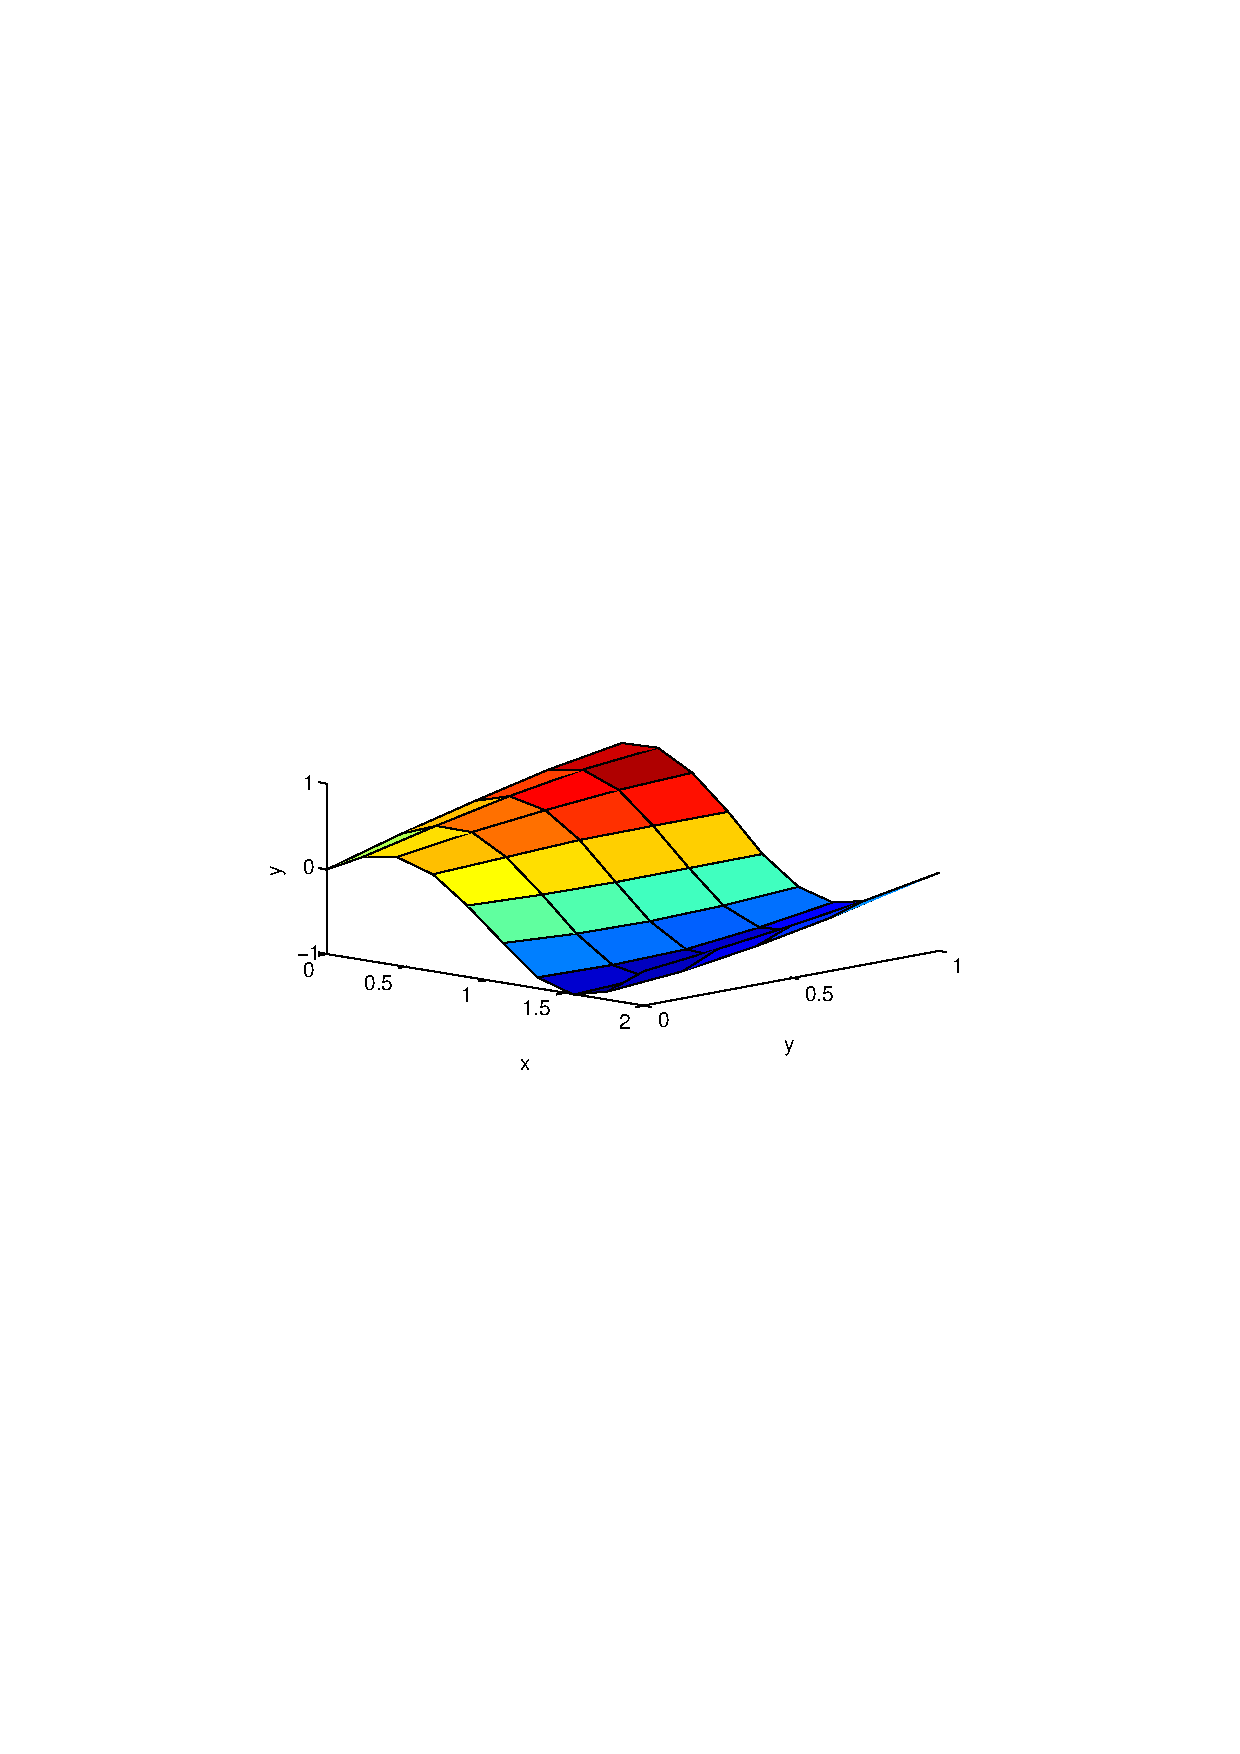
\includegraphics[width=0.45\linewidth, trim=3cm 11cm 3cm 11cm]{figure/X.pdf}
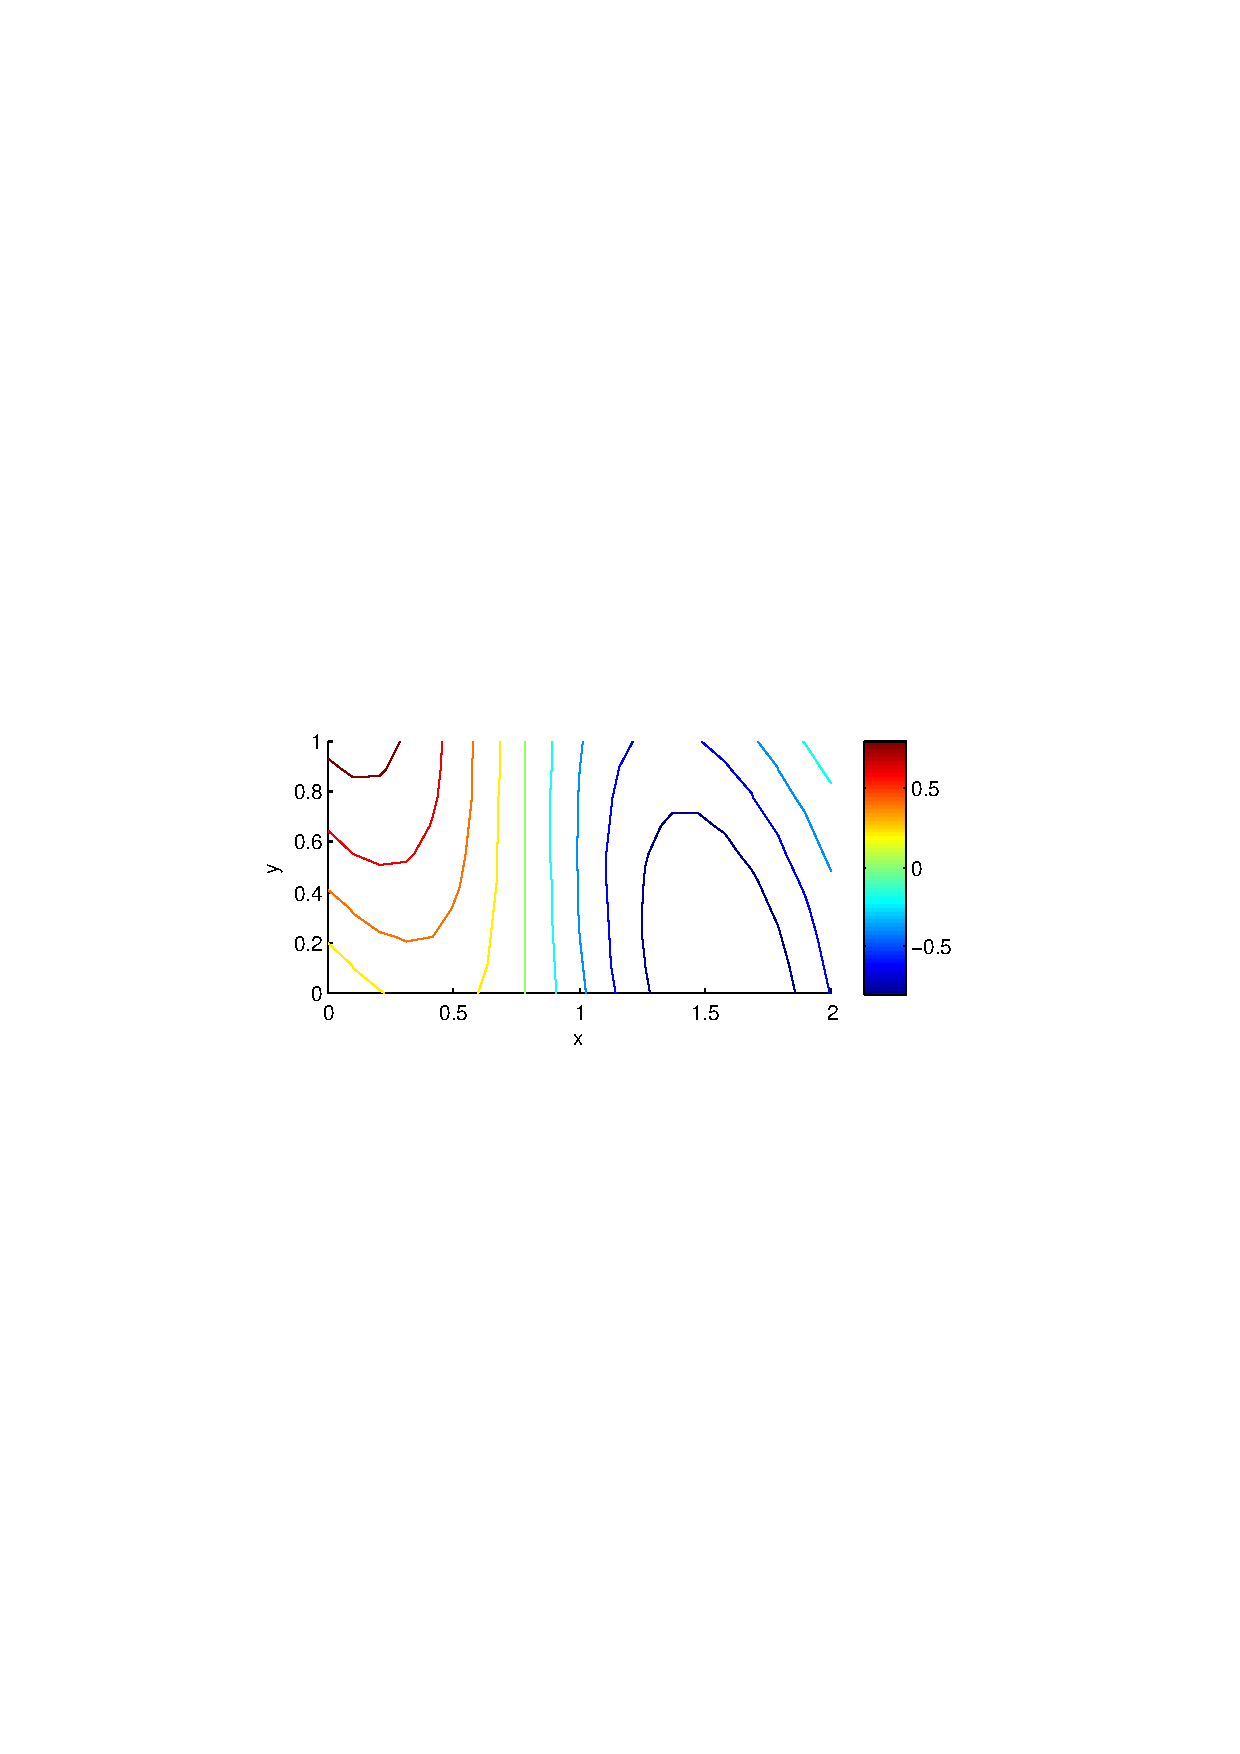
\includegraphics[width=0.45\linewidth, trim=3cm 11cm 3cm 11cm]{figure/Y.pdf}
\caption{Surface and contour plots showing the two dimensional function $z(x,y)=\sin(x+y)\cos(2x)$.}
\end{figure}

\section{Equation}
\begin{equation}
f(t)=\left\{ \begin{array}{ll}
1,~~~~ & t< 1 \\
t^2 & t\geq 1
\end{array}\right.
\end{equation}

\section{Table}
\begin{table}[H]
\centering
\caption{Values of $f(t)$ for $t=0,1,\dots 5$.}
\begin{tabular}{l|llllll} \hline\hline
$t$ & 0 & 1 & 2 & 3 & 4 & 5 \\ \hline
$f(t)$ & 1 & 1 & 4 & 9 & 16 & 25 \\ \hline\hline
\end{tabular}
\end{table}

\section{Chemical structure}
\begin{center}
\chemfig{X*5(-E-T-A-L-)}
\end{center}


\section{Source code listing}
\begin{minted}[frame=single]{matlab}
% Generate x- and y-nodes
x=linspace(0,1); y=linspace(0,1);

% Calculate z=f(x,y)
for i=1:length(x)
 for j=1:length(y)
  z(i,j)=x(i)+2*y(j);
 end
end
\end{minted}

\subsection{Other alternatives to the Theory chapter}
Sometimes, it is more appropriate to name this chapter Background.

At CSE, there exists a large span of different types of thesis works. Sometimes it is more appropriate to join the Theory and Methods chapters, sometimes the Theory chapter would be so small that it should be a subsection. Talk to your supervisor to find the most appropriate structure for your thesis.

% METHODS
% CREATED BY DAVID FRISK, 2016
\chapter{Methods}
Methods text.

% RESULTS
% CREATED BY DAVID FRISK, 2016
\chapter{Results}
Describe you results. Use tables, diagrams etc. for illustration.

% CONCLUSION
% CREATED BY DAVID FRISK, 2016
\chapter{Conclusion}

You may consider to instead divide this chapter into discussion of the results and a summary. 

\section{Discussion}

\section{Conclusion}


% REFERENCES / BIBLIOGRAPHY
\cleardoublepage
\addcontentsline{toc}{chapter}{Bibliography}
% CREATED BY DAVID FRISK, 2016
\begin{thebibliography}{69}

\bibitem{Reference} Frisk, D. (2016) A Chalmers University of Technology Master's thesis template for \LaTeX . Unpublished.

\end{thebibliography}


% APPENDICES
\cleardoublepage
\appendix
\setcounter{page}{1}
\pagenumbering{Roman}			% Capitalized roman numbering starting from I (one)

% CREATED BY DAVID FRISK, 2016
\chapter{Appendix 1}




\end{document}